\section{Spectrum-Mismatch Lower Bound}\label{sec:theorem}

A JEPA whose latent predictor is a unitary map on density matrices faces
a structural obstruction that depends only on spectra. The closed-form
lower bound below characterises the Hilbert--Schmidt training loss of
such a predictor: the bound vanishes if and only if the context and
target density matrices have identical spectra. The main text invokes
this result as a structural diagnostic for the full joint-state unitary
predictor. The practical training objective is reduced and projected,
so the theorem does not transfer as an exact lower bound on the loss
optimised in \cref{eq:jepa-loss}.

\subsection{Setup}\label{sec:theorem-setup}

Let $\mathcal{H} \cong \mathbb{C}^{d}$ with $d = \dtot$ be the joint
system--environment Hilbert space of the architecture introduced in
\cref{sec:architecture}~\cite{nielsen2010quantum,breuer2002theory}, and let $\mathrm{U}(d)$ denote the group of
$d \times d$ unitary matrices. For a Hermitian matrix $A \in \mathbb{C}^{d
\times d}$, write $\lambda^{\downarrow}(A) \in \mathbb{R}^{d}$ for its
eigenvalue vector arranged in non-increasing order. The
Hilbert--Schmidt (Frobenius) norm and inner product are
$\langle A, B \rangle_{F} = \Tr(A^{\dagger} B)$ and
$\lVert A \rVert_{F} = \sqrt{\Tr(A^{\dagger} A)}$.
A JEPA training pair $(\rho_{t}, \rho_{t+k}^{+})$ consists of a context
density matrix $\rho_{t}$, produced by the online encoder from observations
$x_{\leq t}$, and a target density matrix $\rho_{t+k}^{+}$, produced by the
EMA target encoder from observations $x_{\leq t+k}$. The predictor is a
unitary $U^{k} \in \mathrm{U}(d)$ obtained by $k$-fold application of the
one-step unitary in \cref{eq:predictor}, and the full-state matching loss is
\begin{equation}\label{eq:jepa-loss-main}
  \mathcal{L}(U^{k}; \rho_{t}, \rho_{t+k}^{+})
  \;=\;
  \bigl\lVert U^{k} \rho_{t}\, (U^{k})^{\dagger}
              - \rho_{t+k}^{+} \bigr\rVert_{F}^{2} .
\end{equation}

\subsection{Main theorem}\label{sec:theorem-main}

\begin{theorem}[Spectrum-mismatch lower bound]\label{thm:spectrum-mm}
Let $\rho, \sigma \in \mathbb{C}^{d \times d}$ be Hermitian, with sorted
eigenvalue vectors $\lambda^{\downarrow}(\rho), \lambda^{\downarrow}(\sigma)
\in \mathbb{R}^{d}$. Then
\begin{equation}\label{eq:spectrum-mm-main}
  \min_{U \in \mathrm{U}(d)}
  \bigl\lVert U \rho\, U^{\dagger} - \sigma \bigr\rVert_{F}^{2}
  \;=\;
  \bigl\lVert \lambda^{\downarrow}(\rho)
             - \lambda^{\downarrow}(\sigma) \bigr\rVert_{2}^{2},
\end{equation}
and the minimum is attained at any $U^{\star} \in \mathrm{U}(d)$ that maps a
sorted eigenbasis of $\rho$ to a sorted eigenbasis of $\sigma$ in matching
order.
\end{theorem}

\paragraph{Proof} Expand the Frobenius norm as
$\Tr(\rho^{2}) + \Tr(\sigma^{2}) - 2\,\Tr(U \rho U^{\dagger} \sigma)$. The
first two terms are unitary-invariant; minimising the whole is equivalent to
maximising $\Tr(U \rho U^{\dagger} \sigma)$, for which von~Neumann's trace
inequality gives
$\max_{U}\Tr(U\rho U^{\dagger}\sigma) = \sum_{i}\lambda_{i}^{\downarrow}(\rho)\,
\lambda_{i}^{\downarrow}(\sigma)$, with equality when $U$ aligns the sorted
eigenbases. Substituting and collecting terms yields the squared $\ell_{2}$
distance between sorted eigenvalue vectors. Thus the result follows from
von~Neumann's trace inequality on the unitary orbit of~$\rho$ under the
Frobenius objective. It is closely related to Hoffman--Wielandt
eigenvalue-stability bounds~\cite{hoffman1953variation}, but the
optimisation used here is the unitary-orbit trace maximisation.

\subsection{Corollaries}\label{sec:theorem-corollaries}

Two consequences specialise the theorem to JEPA training.

\begin{corollary}[Irreducible JEPA error]\label{cor:irreducible}
For every unitary predictor $U^{k} \in \mathrm{U}(d)$ and every context/target
pair $(\rho_{t}, \rho_{t+k}^{+})$,
\begin{equation}\label{eq:cor-irreducible}
  \mathcal{L}(U^{k}; \rho_{t}, \rho_{t+k}^{+})
  \;\geq\;
  \bigl\lVert \lambda^{\downarrow}(\rho_{t})
             - \lambda^{\downarrow}(\rho_{t+k}^{+}) \bigr\rVert_{2}^{2}.
\end{equation}
\end{corollary}

The right-hand side of~\eqref{eq:cor-irreducible} depends only on spectra and
is independent of $U^{k}$. It therefore cannot be reduced by any training
procedure that optimises only over $\mathrm{U}(d)$. We call this quantity the
\emph{irreducible JEPA error} of the pair $(\rho_{t}, \rho_{t+k}^{+})$.

\begin{corollary}[Orbit-projected target eliminates the floor]%
\label{cor:orbit}
Let $\rho_{t+k}^{+} = V_{+} \Lambda_{+} V_{+}^{\dagger}$ be a spectral
decomposition and let $\Lambda_{t}$ contain the sorted eigenvalues of
$\rho_{t}$. The orbit-projected target
\begin{equation}\label{eq:orbit-proj-main}
  \widetilde{\rho}_{t+k}^{\,+}
  \;:=\;
  V_{+}\, \Lambda_{t}\, V_{+}^{\dagger}
\end{equation}
has $\lambda^{\downarrow}(\widetilde{\rho}_{t+k}^{\,+}) =
\lambda^{\downarrow}(\rho_{t})$, so
$\min_{U} \lVert U\rho_{t} U^{\dagger} - \widetilde{\rho}_{t+k}^{\,+}
\rVert_{F}^{2} = 0$.
\end{corollary}

Orbit projection is the minimal full-state target rewrite that makes
the unitary matching problem reducible. Eigenvectors, which carry the
direction of evolution the predictor must learn, are preserved; only
the spectrum is replaced. The corollary is a mathematical diagnostic
and does not claim that the practical reduced/projected objective
implements orbit projection.

\subsection{Physical meaning}\label{sec:theorem-physical}

Unitary conjugation is an isometry of Hermitian matrices in the
Hilbert--Schmidt inner product, so the image
$U^{k}\rho_{t}(U^{k})^{\dagger}$ lies on the \emph{unitary orbit} of
$\rho_{t}$, a submanifold of density-matrix space parametrised entirely
by the spectrum $\lambda^{\downarrow}(\rho_{t})$. A generic target
density matrix produced by encoding a future observation has a
different spectrum, since the entropy of a realised trajectory is not
the entropy of the uncertainty over trajectories, and therefore lies
on a different orbit. \Cref{thm:spectrum-mm} quantifies the gap: the
closest the predictor's output can get to such a target, over all
unitaries, is the squared $\ell_{2}$ distance between sorted spectra.
Training over $\mathrm{U}(d)$ cannot reduce that floor.

The corollaries describe full-state geometry. They imply nothing about
the spectra of reduced system states or about retention of task
variables by a downstream probe; those empirical questions are
evaluated in the blind-rollout and action-binding experiments.

\subsection{Numerical invariant check}\label{sec:theorem-invariants}

\begin{figure}[t]
  \centering
  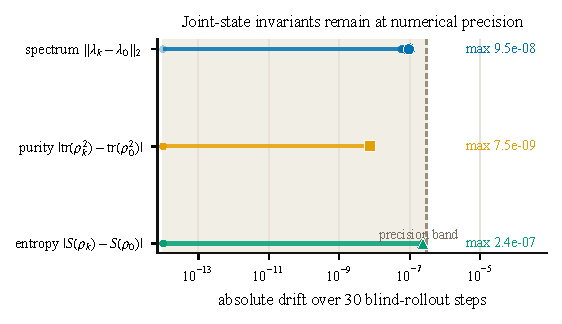
\includegraphics[width=0.72\textwidth]{figures/fig_invariants_verification.pdf}
  \caption{\textbf{Joint-state invariant check.} A trained UWM-JEPA
  predictor preserves spectrum, purity, and entropy under blind rollout
  to floating-point precision. The largest observed drift over
  $30$ steps is below $2.4\times 10^{-7}$, verifying the implemented
  unitary predictor rather than any downstream performance metric.}
  \label{fig:supp-invariants}
\end{figure}
